%%%%%%%%%%%%%%%%%%%%%%%%%%%%%%%%%%%%%%%%%%%%%%%%%%%%%%%%%%%%%%%%%%%%%%%%
%    INSTITUTE OF PHYSICS PUBLISHING                                   %
%                                                                      %
%   `Preparing an article for publication in an Institute of Physics   %
%    Publishing journal using LaTeX'                                   %
%                                                                      %
%    LaTeX source code `ioplau2e.tex' used to generate `author         %
%    guidelines', the documentation explaining and demonstrating use   %
%    of the Institute of Physics Publishing LaTeX preprint files       %
%    `iopart.cls, iopart12.clo and iopart10.clo'.                      %
%                                                                      %
%    `ioplau2e.tex' itself uses LaTeX with `iopart.cls'                %
%                                                                      %
%%%%%%%%%%%%%%%%%%%%%%%%%%%%%%%%%%
%
%
% First we have a character check
%
% ! exclamation mark    " double quote  
% # hash                ` opening quote (grave)
% & ampersand           ' closing quote (acute)
% $ dollar              % percent       
% ( open parenthesis    ) close paren.  
% - hyphen              = equals sign
% | vertical bar        ~ tilde         
% @ at sign             _ underscore
% { open curly brace    } close curly   
% [ open square         ] close square bracket
% + plus sign           ; semi-colon    
% * asterisk            : colon
% < open angle bracket  > close angle   
% , comma               . full stop
% ? question mark       / forward slash 
% \ backslash           ^ circumflex
%
% ABCDEFGHIJKLMNOPQRSTUVWXYZ 
% abcdefghijklmnopqrstuvwxyz 
% 1234567890
%
%%%%%%%%%%%%%%%%%%%%%%%%%%%%%%%%%%%%%%%%%%%%%%%%%%%%%%%%%%%%%%%%%%%
%
\documentclass[12pt,a4paper,final]{iopart}
\usepackage[letterpaper]{geometry}
\newcommand{\gguide}{{\it Preparing graphics for IOP journals}}
%Uncomment next line if AMS fonts required
\usepackage{iopams}  
\usepackage{graphicx}
\usepackage[breaklinks=true,colorlinks=true,linkcolor=blue,urlcolor=blue,citecolor=blue]{hyperref}
%\usepackage[T1]{fontenc}
%\usepackage{alltt}
%\usepackage{underscore}

% Use the following lines to restore the footnote line.
\makeatletter
\def\footnoterule{\kern-3\p@
  \hrule \@width 2in \kern 2.6\p@} % the \hrule is .4pt high
\makeatother

%% Choose Font %%
%\usepackage{fontspec}
%\setmainfont{Fontin}
%\usepackage{libertine}
\usepackage{graphicx}
\usepackage{tabularx}
\usepackage{ltxtable}
\usepackage[colorlinks=true]{hyperref}

\renewcommand{\tabularxcolumn}[1]{>{\small}m{#1}}

\begin{document}

\title{GENIE Systematic Uncertainties with the Multi-universe Approach in CAFAna}

\section{Overview}
The standard approach for drawing the NOvA systematic error band from GENIE cross section models is to vary the GENIE tunable physics parameters by $N$ $\sigma$'s, $N\in\{-2,-1,1,2\}$, input this number through the shift parameter of the CAFAna Spectrum class, and obtain shifted spectra as the boundaries of the error band. There are tens of tunable GENIE parameters, hereafter referred to as GENIE knobs, but only a few of them having the biggest effects are varied. This leaves somewhat arbitrary where to leave out the knobs.

A consistent way of treating the GENIE systematic uncertainties across all analyses, known as the multi-universe approach, was proposed, which varies all the knobs at the same time. One can think of a universe as a collection of physics parameters. Different universes have different values for these physics parameters. One advantage of this approach is it enables bin-to-bin correlation studies which could be in turn followed by dimensionality reduction analyses such as principal component analysis (PCA)~\cite{ref1}.

In this note details of the implementation of this approach under the CAFAna framework is given, followed by sanity checks of this approach compared with the conventional way. Then some known issues are discussed. In the end the computing resources consumed by this class is presented.

\section{Implementation}
The code can be found, under NOvA's offline repository, in \path{CAFAna/XSec/GenieMultiverseSyst.[h,cxx]}. There are several classes defined in the files, where \texttt{MultiverseSpectra} takes on a central role.

Since there are tens of GENIE tunable knobs, to switch the knobs on and off easily, a so called knob configuration file is input into the class with a default name of \texttt{knob\_config.txt} and a default path of the current directory.

With the development of theories, new knobs could be added into GENIE. To account for the possible difference in the tunable parameters used in different production datasets, a script is offered to make a configuration file based on the underlying GENIE versions of the production datasets, located in \path{CAFAna/XSec/Utilities/make_template_knob_config.py}. To use this scrip, simply do:
\begin{enumerate}
  \item setup nova
  \item \texttt{\$ python make\_template\_knob\_config.py -d \textless sam\_defname\textgreater}
\end{enumerate}
This script generates a complete set of GENIE knobs with the name of a knob followed by a number. The names are extracted from the source file \texttt{\$NUTOOLS\_DIR/source/NuReweight/ReweightLabels.h}, with the leading ``\texttt{fReweight}" or ``\texttt{kReweight}" stripped. The number following a knob name assumes 3 numbers, namely 0, 1, or 2. 0 means it is disabled, like it does not exist at all. If it is 1, a random number is drawn from a normal distribution $\mathcal{N}(0,1)$, and used to construct a \texttt{SystShifts} object as an input argument to the \texttt{Spectrum} class. If it is 2, it means the knob chooses between two alternative models. In this case, a random number is drawn from $\{0,1\}$ with equal probability, where 0 represents the nominal model, and 1 represents the alternative model. Note that even for this kind of knobs mode 1 can still be used. In this case CAFAna does a linear evolution from the weight of the first model to that of the second model.

Note that to make the results reproducible, the random seed sequence starts from 1001, leaving the first 1000 numbers to the flux multi-universe~\cite{ref2}.

A default configuration file is available in \path{CAFAna/XSec/Utilities/knob_config.txt}. By and large it enables all available knobs, and uses mode 2 whenever the knob is for alternative models. However, some knobs tune the same physical parameter. For example, \texttt{MaCCQE} tunes the normalization and shape for CCQE at the same time, and \texttt{NormCCQE} and \texttt{MaCCQEshape} tune normalization and shape of CCQE, respectively. To avoid double counting, the three knobs should not be enabled at the same time. According to the former studies~\footnote{Please refer to page 15 in \href{https://nova-docdb.fnal.gov:441/cgi-bin/ShowDocument?docid=15214}{DocDB-15214}.}, decision was made to enable separate knobs and disable the combined one.

\subsection{Interface}
The interface is designed to mimic that of the \texttt{Spectrum} class as close as possible, with two more constructor arguments. One is the number of universes one would like to generate, and the other is the pathname of the knob configuration file. Please consult the \href{http://nusoft.fnal.gov/nova/novasoft/doxygen/html/classana_1_1MultiverseSpectra.html}{doxygen page} for detailed information.

Once you have created a multi-universe object and filled them with the \texttt{SpectrumLoader::Go()} function call, you can start to extract the needed information, namely, the error band.

To obtain the spectrum above the nominal spectrum, use \path{MultiverseSpectra::UpperSigma()}. Similarly, \path{MultiverseSpectra::LowerSigma()} gives you the spectrum below the nominal one. The boundaries of the error band are obtained in the following way. For each bin of the spectrum, each universe has a different number of events. If one plots the distribution of number of events in a bin, usually it is not symmetric. For example, Figure~\ref{fig:recoe} shows the reconstructed neutrino energy with all universes overlaid. If one takes the bin between the blue dashed lines and projects the counts to the y-axis, Figure~\ref{fig:spread} results.

\begin{figure}[h]
  \centering
  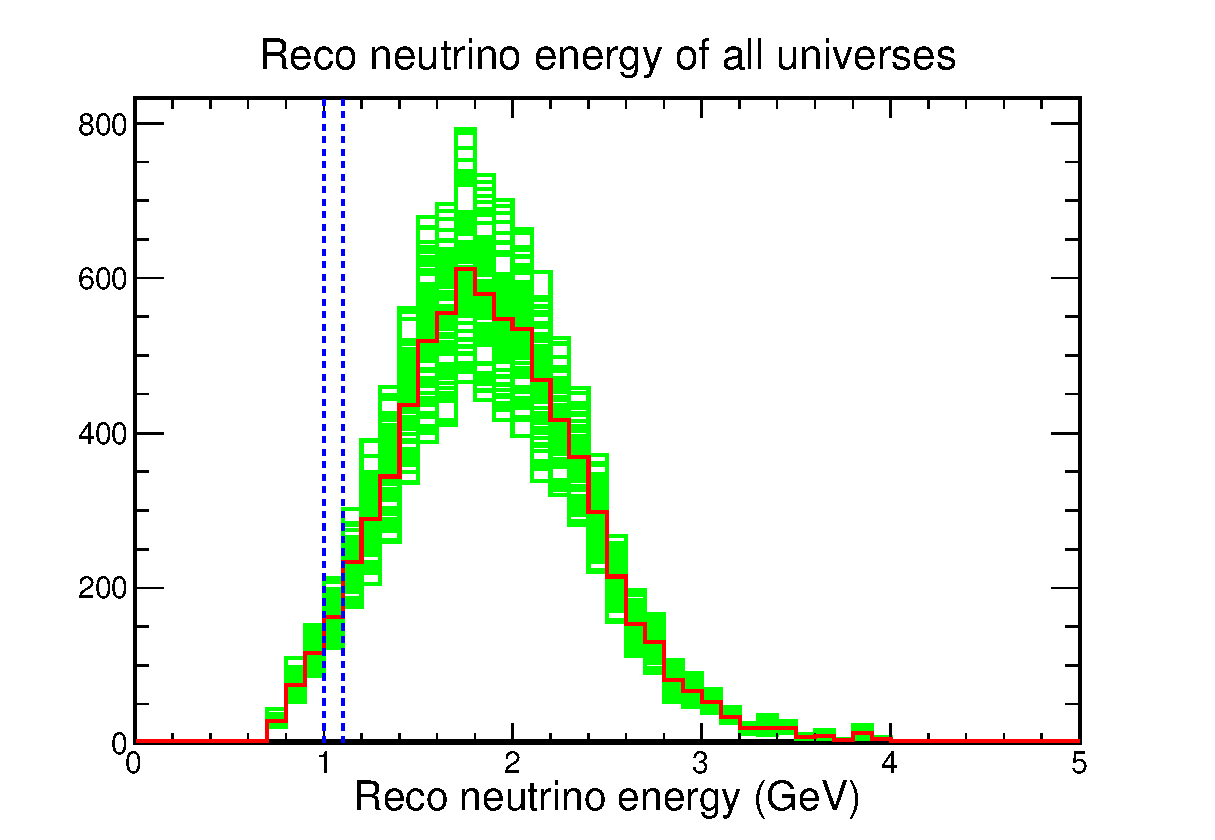
\includegraphics[width=.75\textwidth]{figures/bin_projection.eps}
  \caption{Reconstructed neutrino energy with all universes overlaid. The red histogram represents the nominal universe. To draw the error band, for each bin, project the counts to the y-axis and infer from the distribution.}
  \label{fig:recoe}
\end{figure}

\begin{figure}[h]
  \centering
  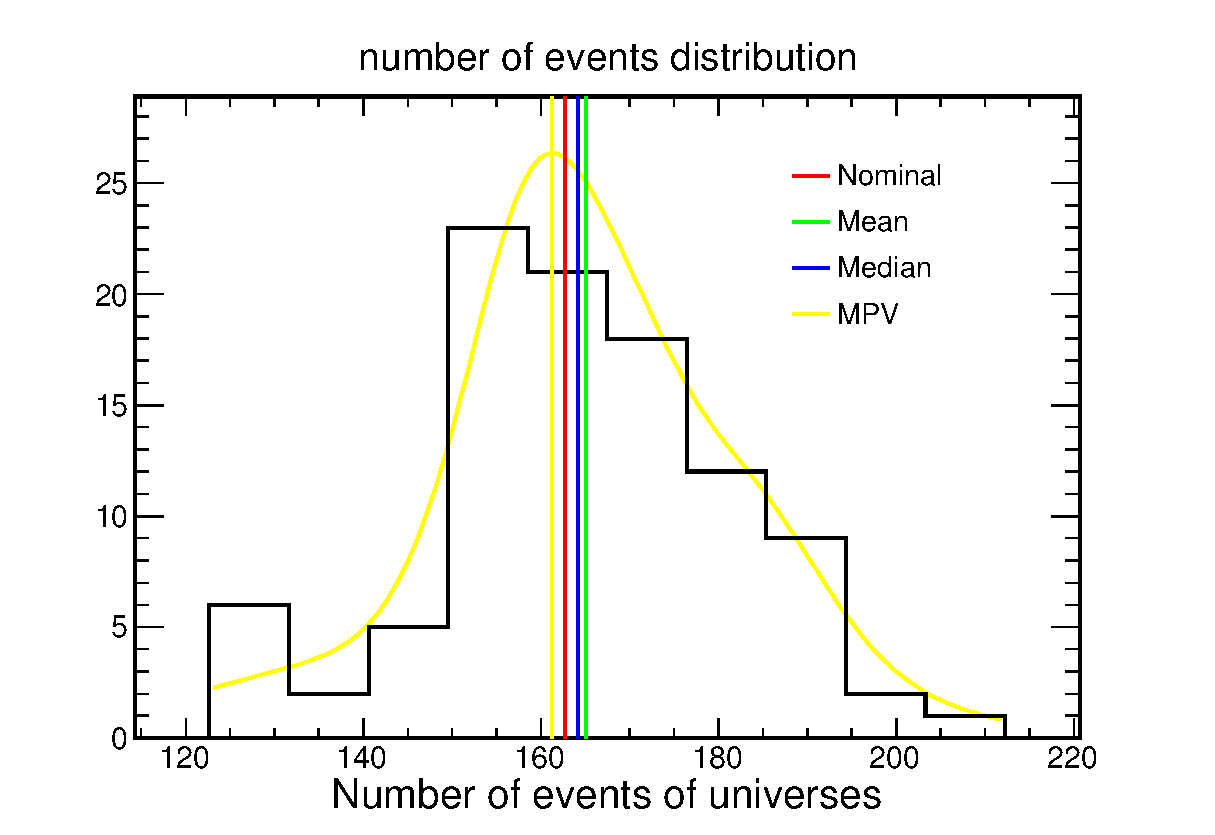
\includegraphics[width=.75\textwidth]{figures/spread_from_different_points.eps}
  \caption{Different choices for the center of the distribution. The nominal value is in red. The mean and the median are drawn from the unbinned sequence of values. For the most probable value (yellow), it is estimated by the Kernel Density Estimation (KDE) algorithm. The yellow curve is the continuous distribution reconstructed by the algorithm.}
  \label{fig:spread}
\end{figure}

\begin{figure}[h]
  \centering
  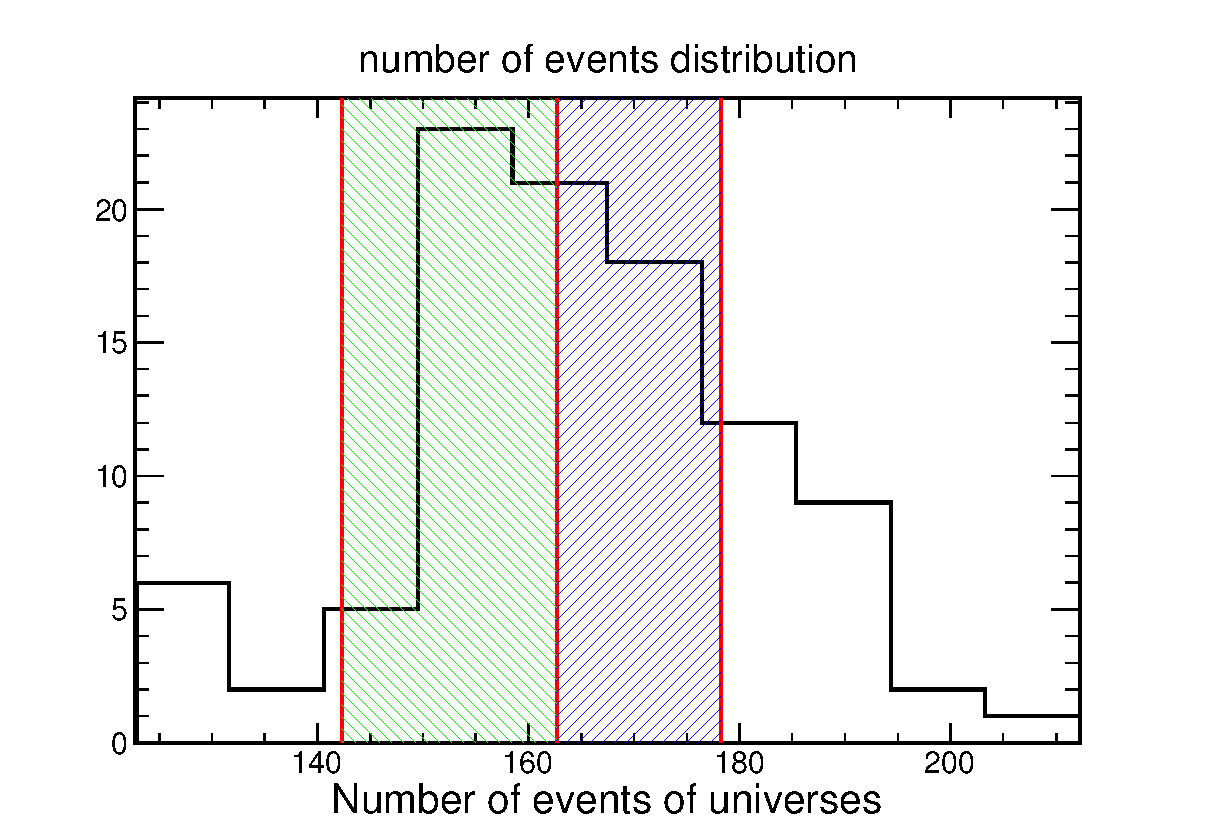
\includegraphics[width=.75\textwidth]{figures/band_boundaries.eps}
  \caption{The upper and lower boundaries of the error band. The boundaries are determined such that the blue and green shaded areas each contain 34\% of the total number of universes.}
  \label{fig:boundaries}
\end{figure}

\begin{figure}[h]
  \centering
  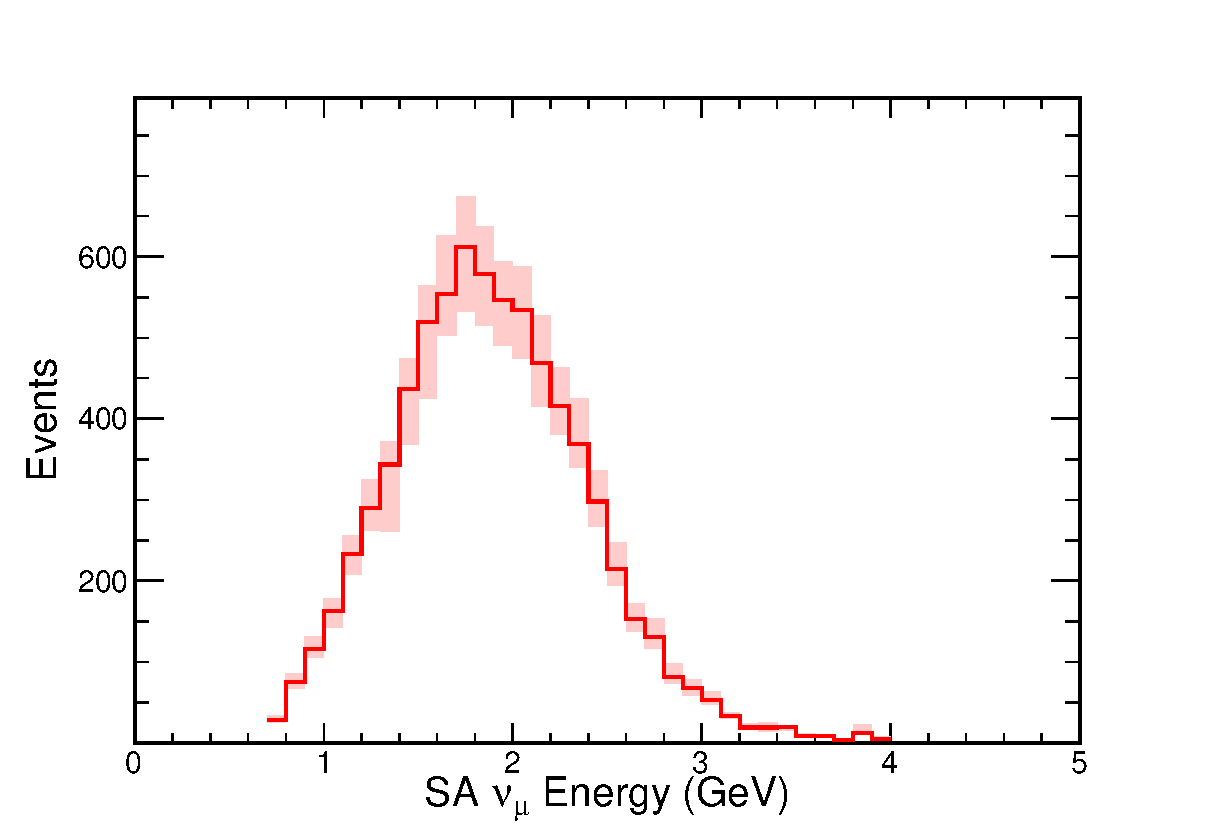
\includegraphics[width=.75\textwidth]{figures/reco_nue_w_error.eps}
  \caption{Error band obtained by this multi-universe approach.}
  \label{fig:reco_nue_w_error}
\end{figure}

The class offers several options for the center of the distribution to draw the spread of the distribution from. Figure~\ref{fig:spread} shows the options to draw the spread from. The default option is set to the nominal value. Once a center is chosen, the upper boundary is drawn from the center such that 34\% of the universes are enclosed in the center line and the upper bound. The lower boundary is obtained in the same way. Figure~\ref{fig:boundaries} shows the boundaries determined by this procedure. Note that the number of universes outside the upper and lower lines are not equal since, in general, the median of the distribution is not the same as the central value you decide to draw the band from. The resulting error band obtained with this approach is shown in Figure~\ref{fig:reco_nue_w_error}.

\section{Performance}
Generating the same number of spectra with this class is significantly slower than generating usual spectra. An investigation was conducted trying to identify the time consuming processes of this class.

\section*{References}
\begin{thebibliography}{10}
  \bibitem{ref1} Bannanje Nitish Nayak, PPFX Systematics, \url{https://nova-docdb.fnal.gov:441/cgi-bin/ShowDocument?docid=18996}
  \bibitem{ref2} Leonidas Aliaga Soplin, G4NuMI/PPFX in NOvA framework, \url{https://nova-docdb.fnal.gov:441/cgi-bin/ShowDocument?docid=16397}
\end{thebibliography}
  
\end{document}